\section{Problema II: Backtracking con poda}

\subsection{Introducción}
Este tipo de solución es utilizando el mismo algoritmo en el paso anterior con alguna que otra modificación a la hora de tomar decisiones
\subsection{Resolución del problema}
La poda que vamos a aplicar es la siguiente, ya que el algoritmo recorre exahustivamente todos los elementos, pero. Resulta que si miramos e mas
detalle, resulta que comparar o buscar una secuencia máxima en una tira de números que nunca puede llegar a superar la máxima encontrada por mas que
se agreguen a todos, no tiene sentido ya que nunca podría superar al máximo por mas que pintemos todos los elementos faltantes por lo tanto ahí podemos parar el
algoritmo.

\begin{algorithm}[H]
\caption{Backtracking}
\begin{algorithmic}[1]
  \Procedure{subSecuRojaMaxima}{\texttt{secu(int): } elementos,\texttt{secu(bool): } validar,\texttt{pila(int): } PilaMaxima,\texttt{pila(int): } Pila,\texttt{int} fin,\texttt{int} it,\texttt{int} n,\texttt{bool} notermine   }
    \State
    \State \While{ (pila $!=$ vacio() $\land$ notermine ) }
    \State losquefaltan $\gets$ fin - it
    \State libres $\gets$ it - pila.size() - 1
    \State \If{libres $>$ losquefaltan}
    \State notermine $\gets$ false
    \State \Else
    \State \While{ (it $<$ fin $\land$ notermine ) }
    \State SecuCreciente(elementos,validar,pila,it,fin)
    \State ..
    \State ..
    \EndIf
    \EndWhile
    \EndIf
    \EndWhile
\end{algorithmic}
\end{algorithm}

Respecto a la complejidad no se debe hacer un análisis exhaustivo debido a que, esta poda en el peor de los casos no resulta efectiva
solamente es útil para los casos promedios, ya que tarde o temprano el algoritmo puede caer en un caso en el que deba recorrer todo el
árbol de soluciones

Solamente hace falta modificar la función ya descripta con anterioridad y su hermana azul.
\newpage
\subsection{Experimentación}
Vamos a utilizar los mismos casos para el ejercicio uno y comparar contra las complejidades del ejercicio uno.
\begin{figure}[h]
    \centering
    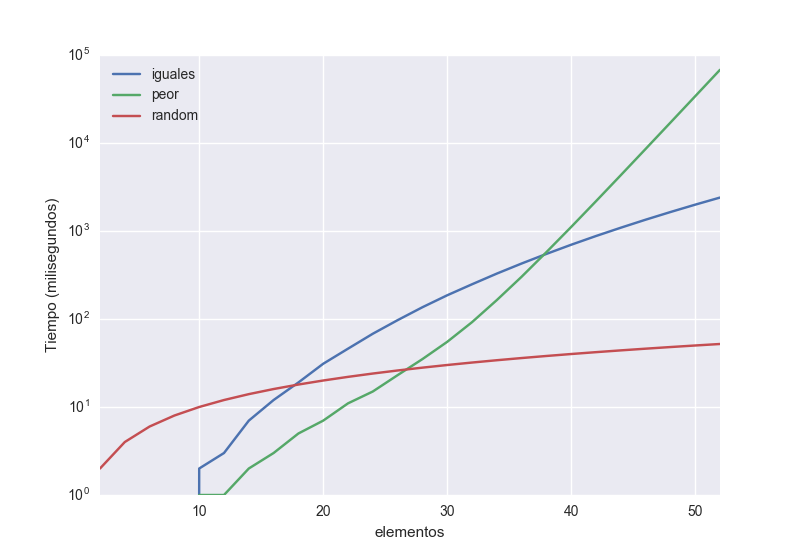
\includegraphics[width=0.55\textwidth]{triple_2.png}
    \caption{Complejidad temporal}
    \label{fig:mesh1}
\end{figure}
Como se ve en la figura 3 nuevamente el peor caso sigue siendo el peor del ejercicio uno , pero ahora se puede apreciar que hay una reducción significativa
del tiempo de cómputo($10^3$), sin embargo el resto de los experimentos se mantuvieron bastante igual, esto sucede porque la poda todo sirve para reducir
tiempo de computo en ciertos casos, pero en el peor de los casos necesariamente tiene que visitar todos los elementos hasta el ultimo. Debido a esto
 la función continua siendo exponencial.
